\subsubsection{\gads}
\label{sec:GALS-DSS}

\figref{fig:GADSS} illustrates the guided local search used instead of random mutation of \garand. \gads finds the best neighbor of a chromosome $Ch_{cur}$ by exhaustively switching two genes with opposite states, and then evaluates the benefit of each swap using \newtext{the Domain Score (DS),} see~\secref{sec:ds}.

\newtext{After found the best neighbor}, \gads keeps the best neighbor $Ch_{BN}$ (i.e. mutation with the most benefit) over the starting chromosome $Ch_{cur}$. If the best neighbor $Ch_{BN}$ improves DS, it then becomes $Ch_{cur}$ the starting point for the next search and the process repeats. 

The search terminates if no improvement is found. The last $Ch_{BN}$ becomes one chromosome in next generation. If the first search iteration does not find any improvement, the search terminates immediately and instead of $Ch_{cur}$ a new random chromosome $Ch_{R}$ is inserted. This increases the random variation and thus the chance to escape a local optimum in the following generation(s). The local search process repeats for each chromosome $Ch0' .. Chn'$. 



\begin{figure}[h]
	\centering
	%\vspace{-10pt}
	\subfloat[GA-LS(DS),GA-LS(AE) ]{
		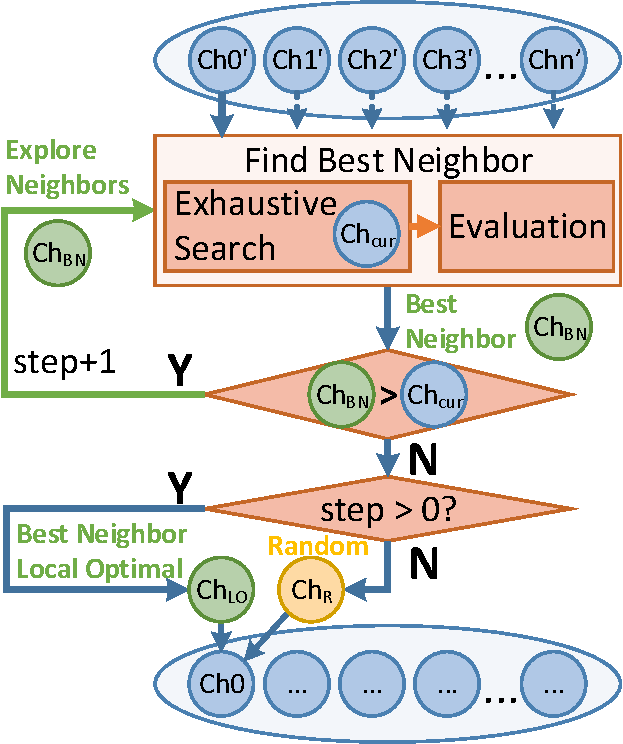
\includegraphics[width=.45\linewidth]{fig/pGADSS.pdf}
		\label{fig:GADSS}}
	\hfill
	\subfloat[GA-LS(Hybrid)]{
		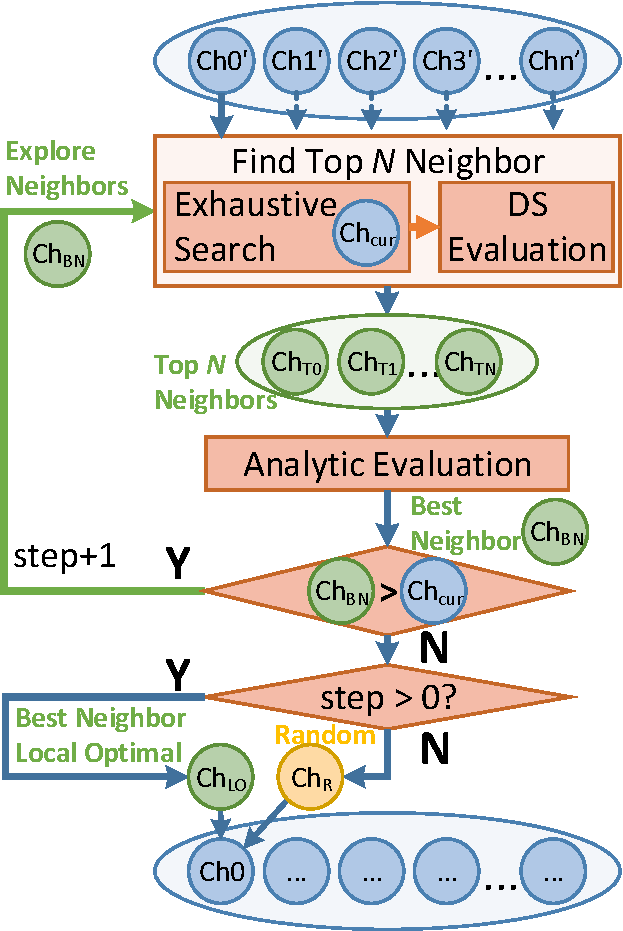
\includegraphics[width=.45\linewidth]{fig/pGADSSA.pdf}
		\label{fig:GAHybrid}}
	%\vspace{-5pt}
	\caption{Guided Local Search}
	%\vspace{-8pt}
\end{figure}

%Local search an iterative algorithm that starts with one solution, then attempts to find the best neighbor solution by exhaustive evaluate all neighbors. If the best neighbor produces a better solution compared with the original one, the best neighbor is made to the new solution, repeating until no further improvements can be found.
%In our GA algorithm, the solution is the chromosome, which defining the domain SW / HW partitioning. The neighbors of the chromosome, are (1) migrating one function type from SW(HW) to HW(SW), and (2) swap a pair of function types between SW and HW.

%Apply local search for each chromosome in generation. Using DSS to evaluate all neighbors of this chromosome, and find the best neighbors as the next step, if it has improvement. Search until no longer improvement. At the end, the mutation finds top 1 candidate (local optimal architecture) for each chromosome to form the new generation.

%If the original chromosome has been evaluated before or it is already the local optimal solution, which local search step is equal to 0, and cannot find a better neighbor in the first step of local search.
%The GA random generated a new chromosome for next generation, to help our GA to explore the large design space with more diversity.

%TODO GS Idea if the best chromosome was created just by cross over. Then, we will discard it with the approach above and replace it with a random chromosome. In effect: the absolute best solution can only be found through mutation in our setting. Improvement: after selection & chross over to a ranking by DS. Top X% of ranked chromosomes are not displaced by random, if no further improvement is found. 




